\documentclass[12pt]{article}

\usepackage{amsmath}
\usepackage{amsfonts}
\usepackage{amssymb}

\usepackage[pdftex]{graphicx}
\usepackage{url}
\usepackage[utf8]{inputenc}

\usepackage{hyperref}
\hypersetup{colorlinks=true}
\input{Qcircuit}

\setlength{\oddsidemargin}{0in}
\setlength{\textwidth}{6.5in}
\setlength{\topmargin}{0in}
\setlength{\textheight}{8.5in}

% These force using more of the margins that is the default style

\begin{document}

% Everything after this becomes content
% Replace the text between curly brackets with your own

\title{Quantum Circuit Simulator for \\
Mobile Devices Running Android OS\\[20pt]
SE 360 Advances In Software Development \\Final Project Proposal}
\author{Mert Can ÇIKLA\\ Izmir University of Economics}

\date{November 8, 2013}

% You can leave out "date" and it will be added automatically for today
% You can change the "\today" date to any text you like
 
\maketitle

% This command causes the title to be created in the document

\section{Introduction}
Quantum computers use the parallel computation power that is hidden
within objects that are governed by quantum physics rather than classic physics.
Due to its power to solve primitive problems such as prime factorization significantly faster 
than current silicon based computers. Quantum computation is getting more and more attention 
every day and its field of research is expanding exponentially. As more people are getting interested in
the topic a tool is needed to make life easier for people who are trying to learn and study quantum 
computation and quantum information processing.\\
 
 With these in mind the proposed plan is to build an application that can simulate 
quantum circuits and runs on the widely popular Android mobile operating system. 

\subsection{Target Devices}
Mobile devices that are running Android 3.0 or above such as tablets or cellphones with a screen larger than ~5 inches.
\subsection{Target Users}
Students studying mathematics, physics or computer engineering is the main 
targeted user group of this application however it might be a useful tool for researchers and professionals aswell.

\section{Application Description}
\begin{figure}[!]
\begin{center}
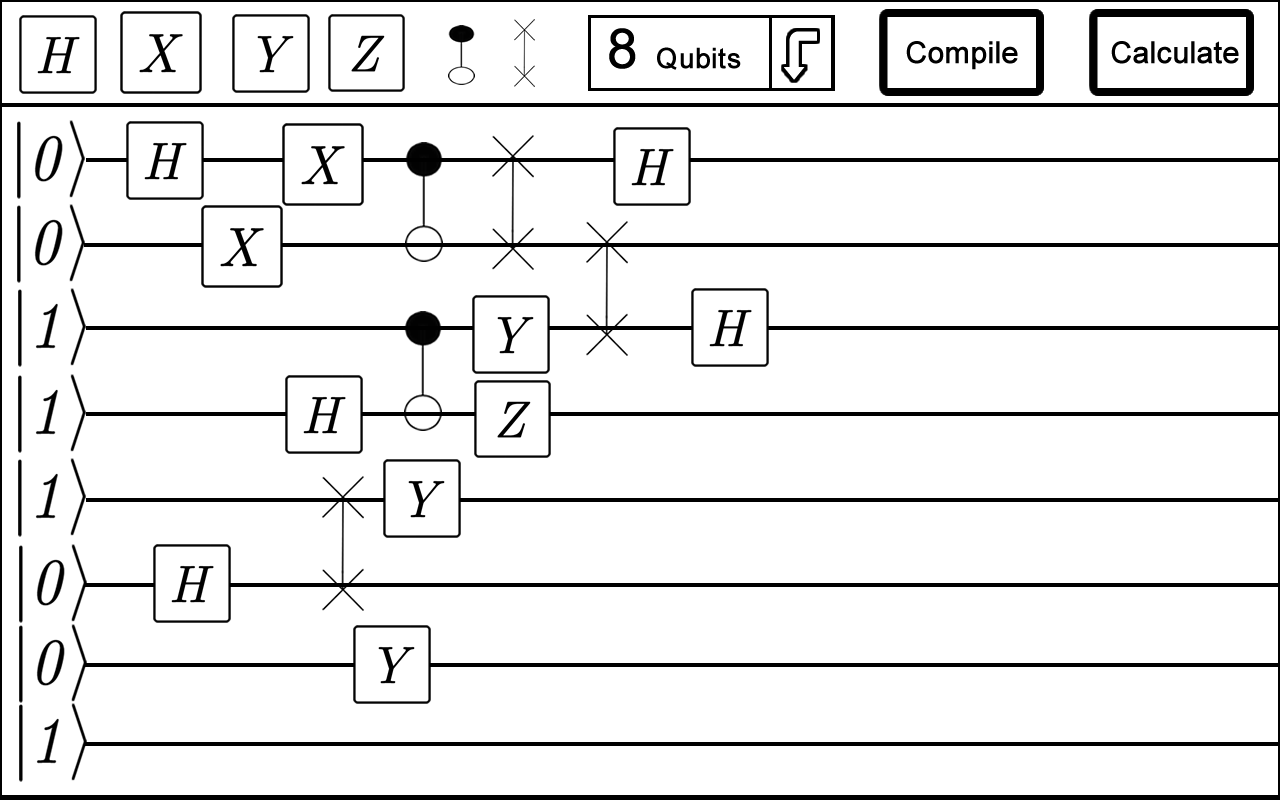
\includegraphics[scale=0.20]{ui}
\end{center}
\caption{Sample user interface envisioned for the application.}
\end{figure}
			\\A quantum gate is represented with a square matrix that has size $2^n$ where $n$ is the number of 
qubits the gate takes as input. A qubit is represented as a 2D vector. Both the gate matrix and 
qubit vector has complex entries.\\
\begin{center}
\resizebox{5cm}{!} {

\begin{tabular}{ l | r }

H & \Qcircuit @C=0.5em @R=.5em @! {\qw & &\gate{H} & \qw }\\
\hline
X & \Qcircuit @C=0.5em @R=.5em @! {\qw & & \gate{X} & \qw }\\
\hline
Y & \Qcircuit @C=0.6em @R=.6em @! {\qw & & \gate{Y} & \qw }\\
\hline
Z & \Qcircuit @C=0.6em @R=.6em @! {\qw & & \gate{Z} & \qw }\\

\end{tabular}

}
\resizebox{5cm}{!} {
\begin{tabular}{ l | r }

CNOT & \Qcircuit @C=1em @R=1.5em { \qw  && \targ & \qw \\
			\qw & & \ctrl{-1} & \qw}\\
\hline
Swap & \Qcircuit @C=1.5em @R=2em  {\qw && \qswap & \qw \\
 \qw && \qswap\qwx  & \qw}\\

\end{tabular}
}\\[5pt]
\textit{Gates and their representations}
\end{center}\\[20pt]
			On top of the application is the toolbar where the basic gates such as Hadamard,Pauli-X,
 Pauli-Y, Pauli-Z, Swap and Cnot are. Next to the gates is there is a spinner that lets 
 the user select how many qubits he/she would like to work on. The qubits will start with 
 state   $\vert 0  \rangle$  and on click will swap to  $\vert 1 \rangle$ and go back to 
 state  $\vert 0 \rangle$  with the second click. The gates on the toolbar can be dragged 
 and dropped to the main area where the circuit will be defined. Gates can be removed from 
 the circuit by dragging them back to the toolbar. By clicking a button on the toolbar the 
 calculation will start and multiply the qubit which is represented by a 2D vector with 
 complex entries. Gates are represented with matrices with dimensions $2^n x 2^n$ where $n$ is the number of 
	qubits the gate takes as input. The result of this multiplication is the 2D output vector. An example of such operation is
 shown below.

$$
\ket{0} =   
 \begin{bmatrix} 
 1 \\[5pt] 
 0
 \end{bmatrix}, H =
\begin{bmatrix} 
 \frac{1}{\sqrt{2}} &  \frac{1}{\sqrt{2}} \\[5pt] 
 \frac{1}{\sqrt{2}} &  \frac{-1}{\sqrt{2}}
 \end{bmatrix}\\[5pt]
$$

\begin{center}
\textit{Hadamard transformation $H$ applied to the given qubit in state $\ket{0}$}
\end{center}
$$
\\[5pt]
H\ket{0} =
\begin{bmatrix} 
 \frac{1}{\sqrt{2}} &  \frac{1}{\sqrt{2}} \\[5pt]  
 \frac{1}{\sqrt{2}} &  \frac{-1}{\sqrt{2}}
 \end{bmatrix}
\begin{bmatrix} 
 1 \\[5pt] 
 0
 \end{bmatrix}
= \begin{bmatrix} 
  \frac{1}{\sqrt{2}} \\[5pt] 
  \frac{-1}{\sqrt{2}}
 \end{bmatrix}
=\frac{1}{\sqrt{2}} \ket{0} +  \frac{-1}{\sqrt{2}}\ket{1}
$$

Quantum computations are done in complex plane and in order realize 
gates that have complex entries such as the Pauli-Y gate shown in Figure 2.
\href{commons.apache.org/proper/commons-math/userguide/complex.html}{Apache Commons Mathematics Library for Complex Numbers}
 will be used.
\begin{figure}[h]
$$ Y =
\begin{bmatrix} 
 0 &  -i \\[5pt] 
 i &  0
 \end{bmatrix}\\[5pt]
$$
\begin{center}
\caption{Pauli-Y gate}
\end{center}
\end{figure}\\

After the computation a list will be shown to the user with $2^n$ entries which are\\ probability amplitudes of every state qubit can be measured in. 
The list will extend beyond the screen size but will be scrollable vertically.

\section{Objectives}
There are 3 main objectives of this project apart from not missing the deadline and providing a bug-free, working application.
\subsection{Ease of Use}

First of all application will be fairly easy to use with a clean and simple GUI. Drag/drop which is an intuitive action on a touch screen will be implemented with the framework included in Android API 11. 

\subsection{Functionality}

This project aims to be able to simulate behaviour of any quantum 
gate or circuit that acts on up to 8 qubits or possibly less depending on screen resolution
of the device running.
\subsection{Scalability}

Users will be able to compile the current circuit into a newly composed gate that is reusable. A new gate icon will
be generated on the toolbar for use. 


\end{document}

